\subsection{Implementation}
To use the camera we created two classes: the Camera and the CameraManager 
classes. The Camera class is the actual camera that moves around and updates 
its model matrix. The CameraManager is used as a proxy for interacting with 
the Camera class. Other classes, like the SDLRenderer class, can use the 
CameraManager class to call the camera's resize method once the resize event 
has been called, as shown in \cref{fig:renderer-resize}.

\begin{figure}[H]
    \centering
    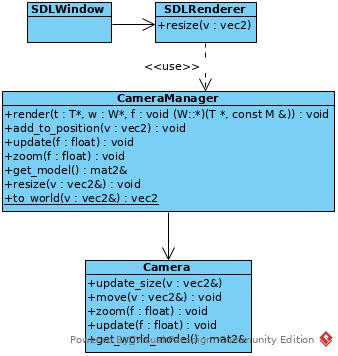
\includegraphics[scale=0.75]{res/renderer-resize.png}
    \caption{Resizing the window.}\label{fig:renderer-resize}
\end{figure}

The only thing the Camera class needs to do is update it's model matrix and 
the matrix that is while rendering objects in the world. The matrix that is 
used for rendering objects in the world is actually the camera's translation 
matrix with the coordinates flipped from positive to negative (or vice-versa)
, multiplied by the inverse of the camera's scaling matrix.
This can be represented by:

$$ rendering\_matrix = (-1 \cdot translation) \cdot scale^{-1} $$

The translation matrix needs to be multiplied by -1, since the world actually 
moves in the opposite direction of the camera.

Every update cycle we also call the CameraManager::update method. This method 
checks the mouse position and adds the corresponding movement vector to a 
buffer. When all four edges have been checked, and the distance moved is 
greater than zero, we add this movement vector to the camera's movement 
buffer. This movement buffer gets multiplied by the difference in time since 
the last update, so that someone on a faster cpu won't actually move faster 
than someone on a slower cpu. Then we check whether we went out of the world's 
bounds, and if so, we correct the camera's position while also taking into 
account the amount of zooming (scaling). This code is shown in 
\cref{lst:camera-update}.

\begin{lstlisting}[caption={Camera update method.},label={lst:camera-update}]
void Camera::update(float delta) {
    vec2 delta_move = _movement_buffer * delta;
    _position += delta_move;
    _movement_buffer = vec2();

    vec2 top_left = (_world_rectangle[0] * get_translation()),
        bottom_right = (_world_rectangle[2] * get_translation()) * _scale.inverse();
    if(top_left.x < 0) {
        _position.x = 0;
    }
    if(top_left.y < 0) {
        _position.y = 0;
    }
    if(bottom_right.x > world_size.x) {
        float new_x = world_size.x - (bottom_right.x - top_left.x);
        _position.x = new_x - 1;
    }
    if(bottom_right.y > world_size.y) {
        float new_y = world_size.y - (bottom_right.y - top_left.y);
        _position.y = new_y - 1;
    }
    update_all();
}
\end{lstlisting}

The update\_all() call at the end updates the camera's matrices.

